\section{Evaluation}
\label{sec:eval}

\iffalse
\begin{figure}[t]
\centering
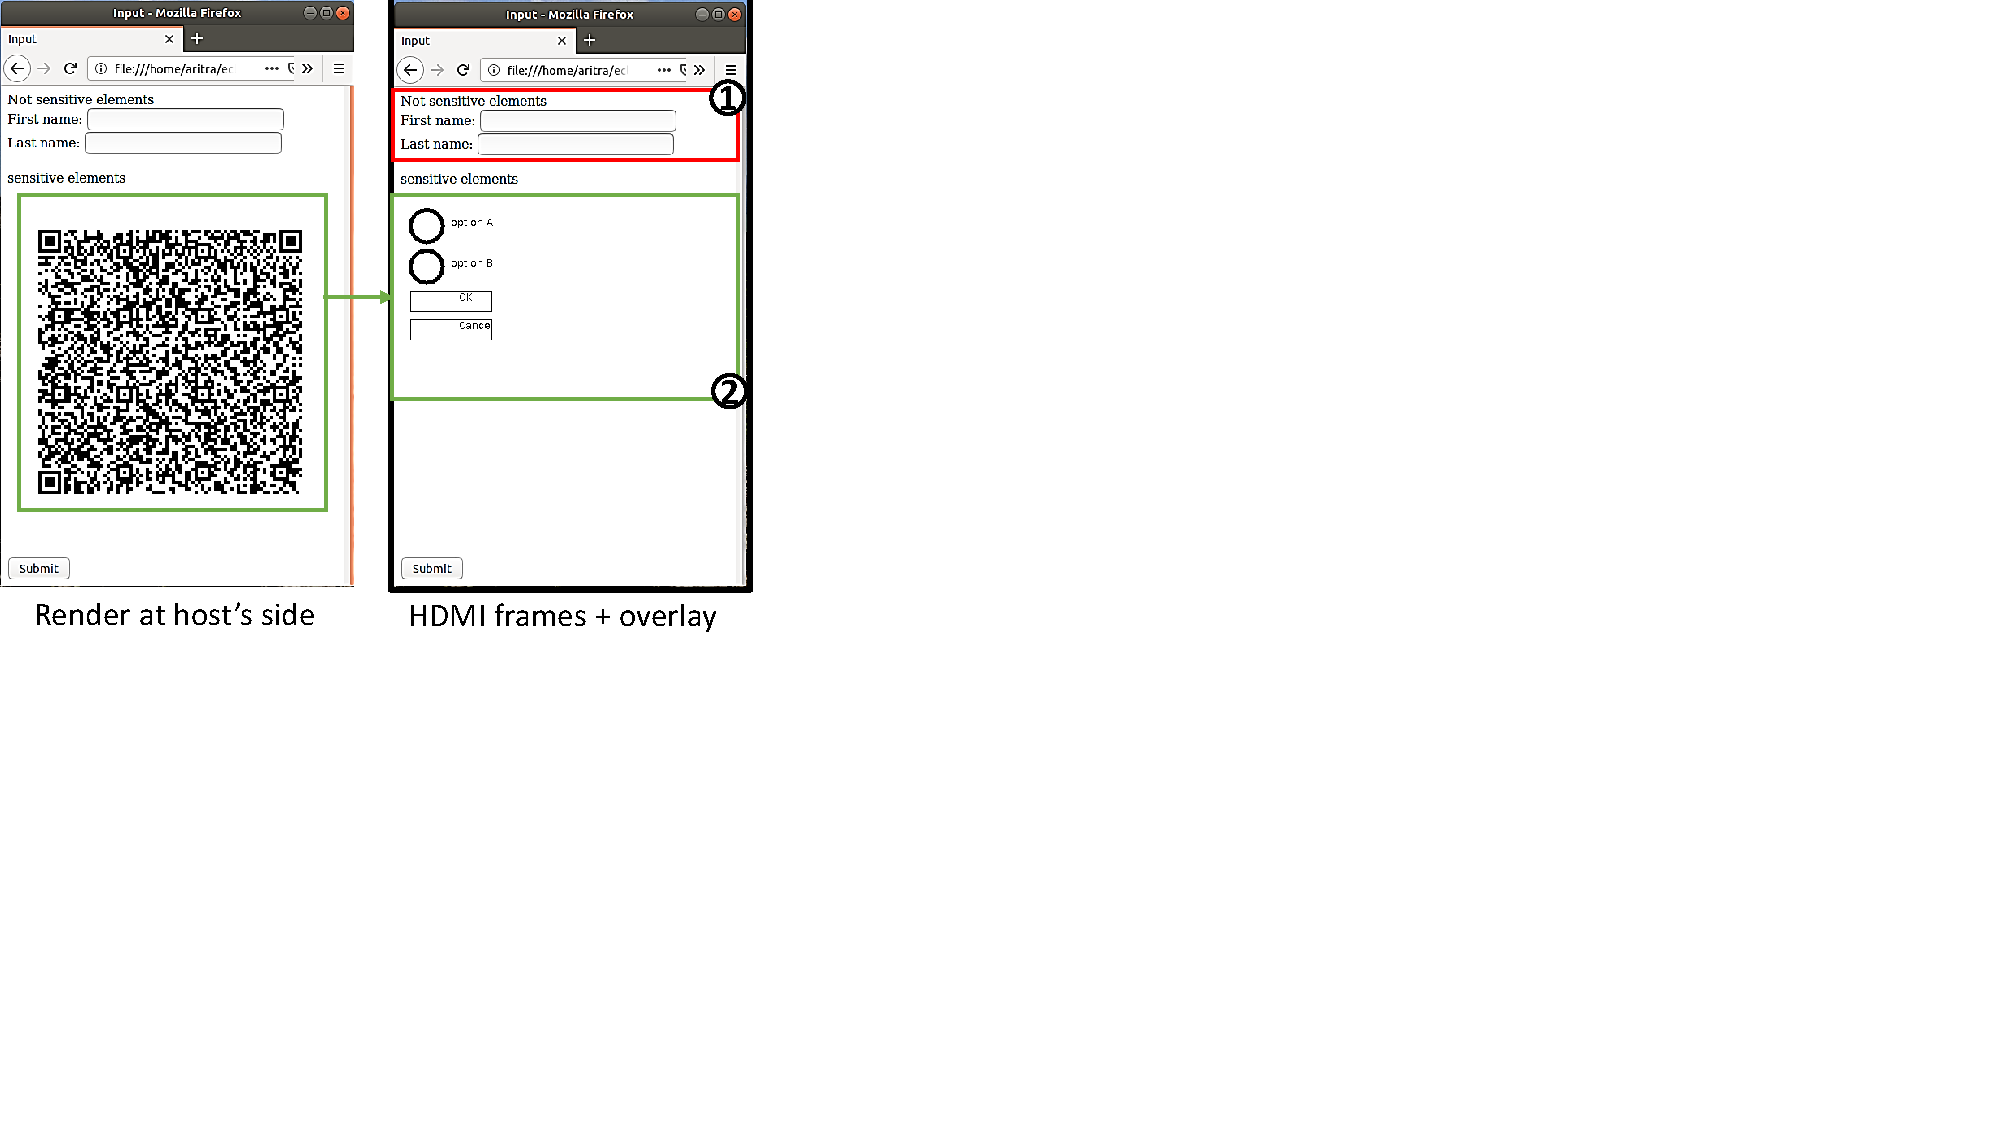
\includegraphics[trim={0 11cm 19cm 0}, clip, width=\linewidth]{overlayScreenShot.pdf}
\caption{\textbf{\name overlay}. }
\label{fig:screenshot_1}
\centering
\end{figure}
\fi



\begin{figure}[t]
\centering
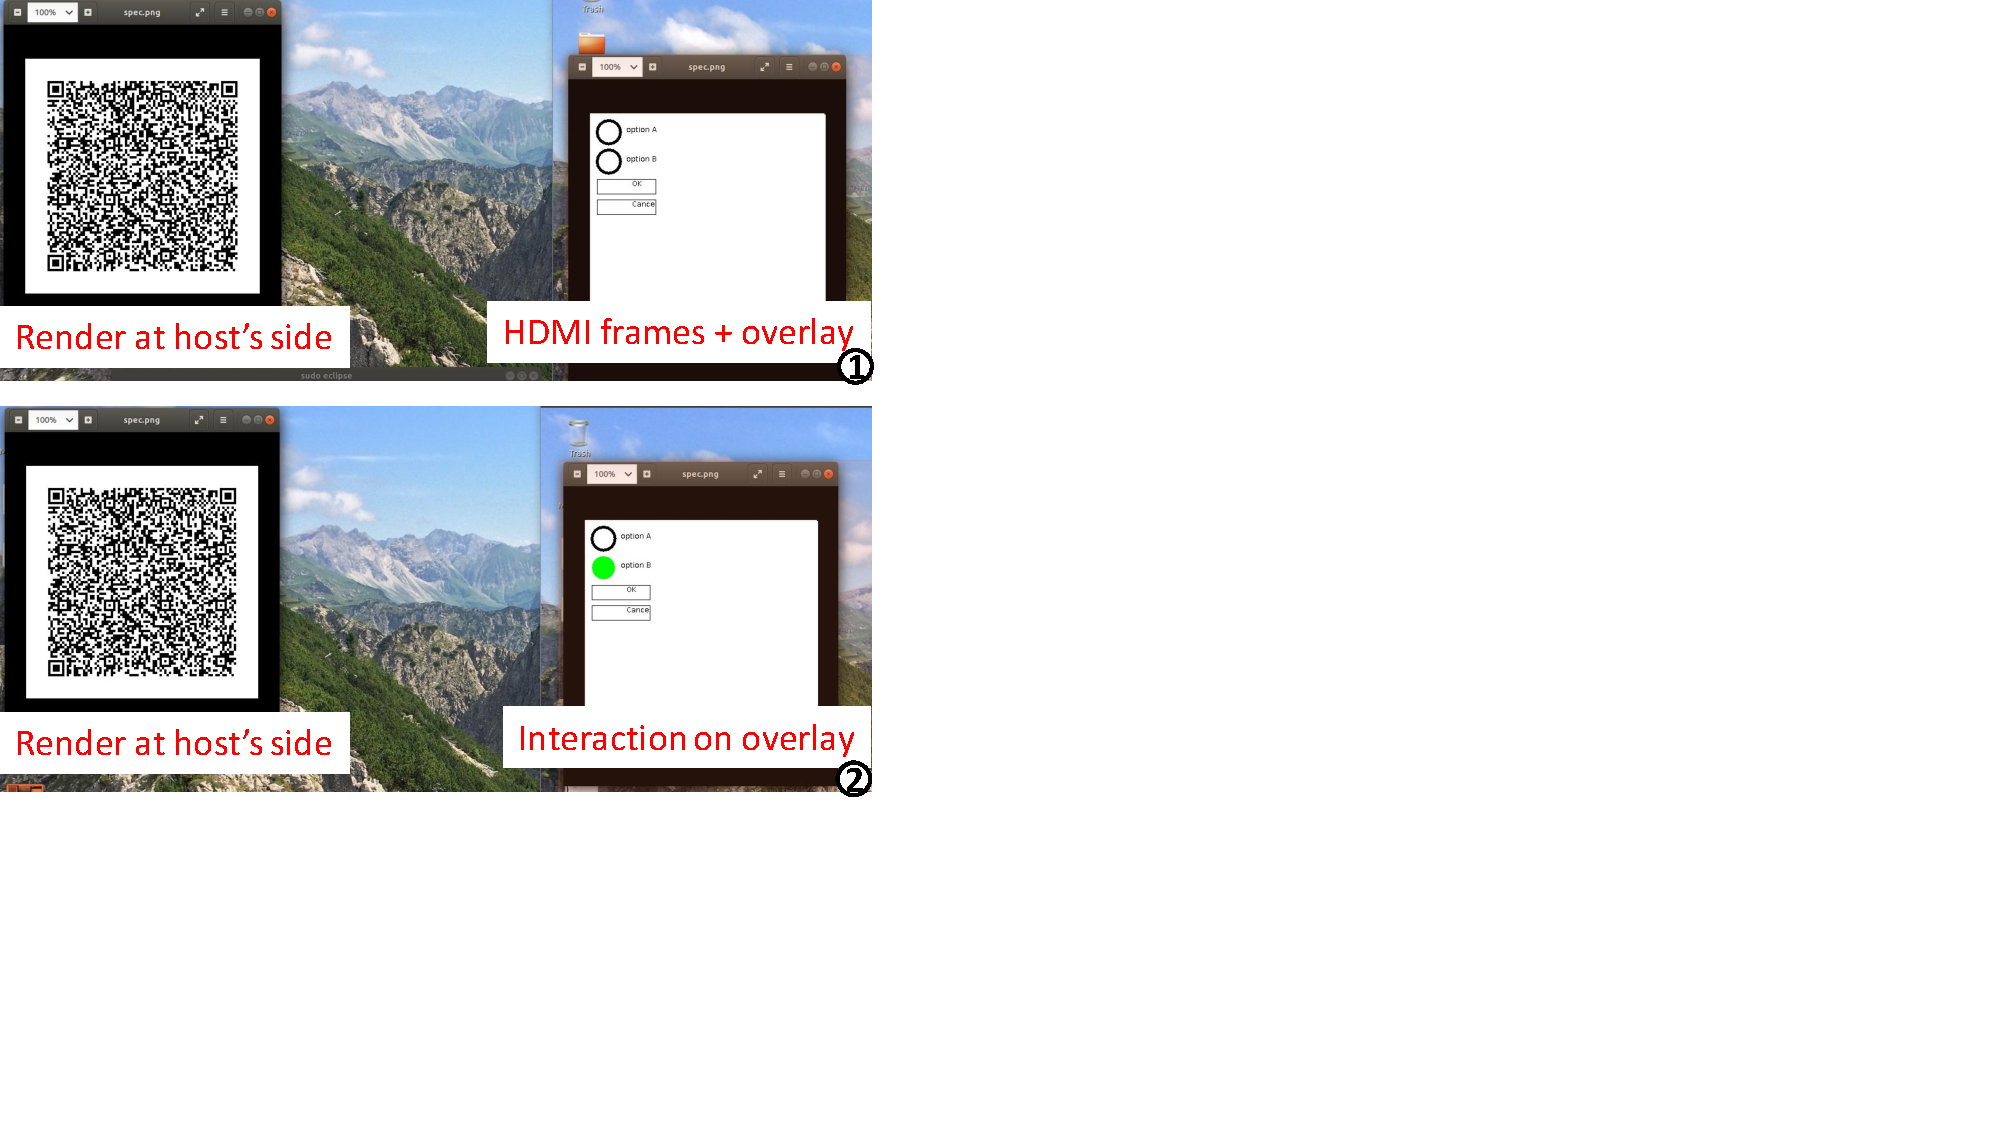
\includegraphics[trim={0 6cm 19cm 0}, clip, width=\linewidth]{activityScreenShot.pdf}
\caption{\textbf{\name overlay}. \one shows the QR code that is visible at the host's side, but the user sees the sensitive form that is overlaid by the \device. \two show a user interaction with the overlaid UI where the user hovers on a specific option on the form. It results in UI reaction, providing the user look and feel of a normal UI. Note all such interactions are executed on the \device, hence completely oblivious to the host.}
\label{fig:screenshot_2}
\centering
\end{figure}


\subsection{Performance}